%%%%%%%%%%%%%%%%%%%%%%%%%%%%%%%%%%%%%%%%%%%%%%%%%%%%%%
% A Beamer template for University of Wollongong     %
% Based on THU beamer theme                          %
% Author: Qiuyu Lu                                   %
% Date: July 2024                                    %
% LPPL Licensed.                                     %
%%%%%%%%%%%%%%%%%%%%%%%%%%%%%%%%%%%%%%%%%%%%%%%%%%%%%%
% Customized for Sharif University of Technology     %
%%%%%%%%%%%%%%%%%%%%%%%%%%%%%%%%%%%%%%%%%%%%%%%%%%%%%%


\documentclass[serif, aspectratio=169]{beamer}
%\documentclass[serif]{beamer}  % for 4:3 ratio
\usepackage[T1]{fontenc} 
\usepackage{fourier} % see "http://faq.ktug.org/wiki/uploads/MathFonts.pdf" for other options
\usepackage{hyperref}
\usepackage{latexsym,amsmath,xcolor,multicol,booktabs,calligra}
\usepackage{graphicx,pstricks,listings,stackengine}
\usepackage{lipsum}
\usepackage[normalem]{ulem}
\usepackage{caption}
\usepackage{tikz}

\author{Ali Sharifi-Zarchi}
\title{Machine Learning (CE 40717)}
\subtitle{Fall 2025}
\institute{
    CE Department \\
    Sharif University of Technology
}
%\date{\small \today}
% \usepackage{UoWstyle}
\usepackage{SUTstyle}

% defs
\def\cmd#1{\texttt{\color{red}\footnotesize $\backslash$#1}}
\def\env#1{\texttt{\color{blue}\footnotesize #1}}
\definecolor{deepblue}{rgb}{0,0,0.5}
\definecolor{deepred}{RGB}{153,0,0}
\definecolor{deepgreen}{rgb}{0,0.5,0}
\definecolor{halfgray}{gray}{0.55}

\lstset{
    basicstyle=\ttfamily\small,
    keywordstyle=\bfseries\color{deepblue},
    emphstyle=\ttfamily\color{deepred},    % Custom highlighting style
    stringstyle=\color{deepgreen},
    numbers=left,
    numberstyle=\small\color{halfgray},
    rulesepcolor=\color{red!20!green!20!blue!20},
    frame=shadowbox,
}
\captionsetup{labelformat=empty}

\begin{document}

\begin{frame}
    \titlepage
    \vspace*{-0.6cm}
    \begin{figure}[htpb]
        \begin{center}
            
\includegraphics[keepaspectratio, scale=0.25]{pic/sharif-main-logo.png}
        \end{center}
    \end{figure}
    \vfill % This pushes the next content to the bottom
    \vspace{-0.35cm}
    % \centering\textit{\tiny Most slides are adapted from Dr. Mahdie Soleymani's ML course}
\end{frame}

\begin{frame}    
\tableofcontents[sectionstyle=show,
subsectionstyle=show/shaded/hide,
subsubsectionstyle=show/shaded/hide]
\end{frame}


\section{Introduction}

\begin{frame}{Binary Classification Problem}
    \begin{itemize}
        \item Consider a \textbf{binary classification} task:
        \begin{itemize}
            \item Email classification: Spam / Not Spam
            \item Online transactions: Fraudulent / Genuine
            \item Tumor diagnosis: Malignant / Benign
        \end{itemize}
    \end{itemize}

    \vspace{0.5em}
    Define the target variable formally:
    \[
        y \in \{0, 1\}, \quad
        \begin{cases}
            0 & \text{Negative class (e.g., benign tumor)}\\
            1 & \text{Positive class (e.g., malignant tumor)}
        \end{cases}
    \]
\end{frame}

\begin{frame}{Linear Regression for Classification}
    \begin{itemize}
        \item A natural approach is to use linear regression:
        \[
            h_\theta(x) = \theta_0 + \theta_1 x
        \]
        and define a threshold at $0.5$ for prediction:
        \[
            \hat{y} =
            \begin{cases}
                1, & h_\theta(\mathbf{x}) \ge 0.5\\
                0, & h_\theta(\mathbf{x}) < 0.5
            \end{cases}
        \]
    \item Here, $\hat{y}$ is the \textbf{predicted class label} (i.e., the model's guess for $y$). It converts the continuous output of $h_\theta(\mathbf{x})$ into a discrete class (0 or 1).
    \end{itemize}

    \vspace{0.5em}
    \begin{minipage}{0.48\linewidth}
        \centering
        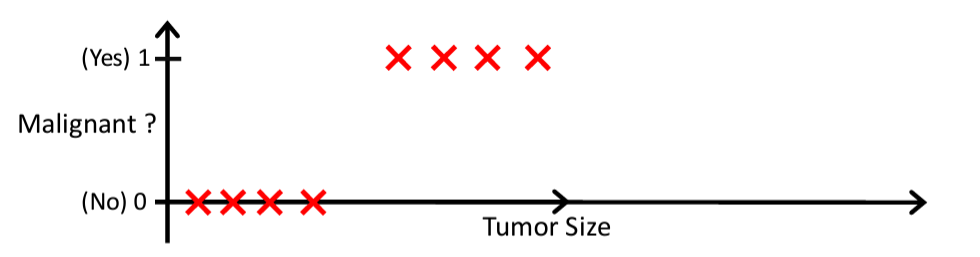
\includegraphics[width=\linewidth]{pic/lrClassification1.png}
    \end{minipage}
    \hfill
    \begin{minipage}{0.48\linewidth}
        \centering
        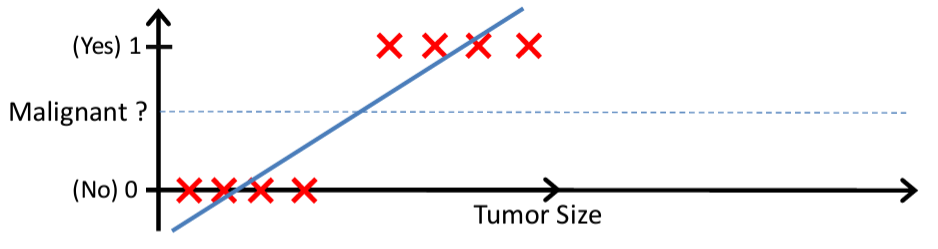
\includegraphics[width=\linewidth]{pic/lrClassification3.png}
    \end{minipage}
\end{frame}

\begin{frame}{Limitations of Linear Regression for Classification}
    \begin{itemize}
        \item The model's output, $h_\theta(\mathbf{x})$, is unbounded and can produce predictions greater than 1 or less than 0.
        \item Linear regression does not provide probabilistic outputs.
        \item The decision boundary may be highly sensitive to outliers.
    \end{itemize}

    \vspace{0.5em}
    \centering
    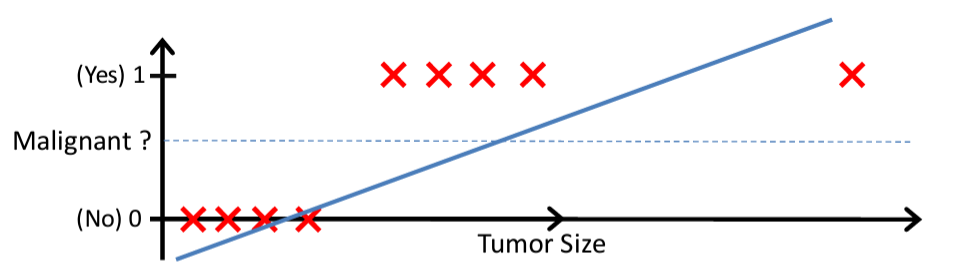
\includegraphics[width=0.68\linewidth]{pic/lrClassification2.png}

    \[
        \text{Requirement: } 0 \le h_\theta(\mathbf{x}) \le 1
    \]

\end{frame}

\begin{frame}{Limitations of Perceptron with Step Activation for Classification}
    \begin{itemize}
        \item As we saw earlier, perceptron Uses a step activation 
        \[
            f(z) =
            \begin{cases}
                1, & z \ge 0\\
                0, & z < 0
            \end{cases}
        \]
        \item The step function has \textbf{slope = 0} almost everywhere (non-differentiable at 0).
        \item No gradient means it cannot use gradient-based optimization.
        \item Produces hard class labels (0/1), not probabilities, thus we cannot measure model confidence — probabilistic outputs are preferred.

    \end{itemize}
\end{frame}

\begin{frame}{Properties of a Good Classifier}
     Therefore, we prefer a model that:
        \begin{itemize}
            \item Outputs \textbf{probabilities} for each class, so it has \textbf{bounded outputs} in $[0, 1]$, making it less sensitive to outliers.
            \item \textbf{Shows model confidence} through its probabilistic output.
            \item Has a \textbf{differentiable, convex objective with non-zero derivative}, allowing efficient optimization with gradient-based methods.
        \end{itemize}
\end{frame}



% \begin{frame}{Limitations of Linear Regression for Classification}
%     \begin{itemize}
%         \item We use the \textbf{sigmoid (or logistic) function}, $\sigma(z)$, to map outputs to $[0, 1]$:

%     \[
%         \sigma(z) = \frac{1}{1+e^{-z}}
%     \]
%     \[
%         \text{Logistic regression hypothesis: } f(x;\mathbf{w}) = \sigma(\mathbf{w}^\top x)
%     \]
%     \end{itemize}
% \end{frame}


%%%% 5 %%%%%
\begin{frame}{Introduction}
    % \begin{itemize}
    %     \item Logistic regression is a \textbf{discriminative} approach.
    % \end{itemize}
    % \begin{figure}[h]
    %   \centering
    %   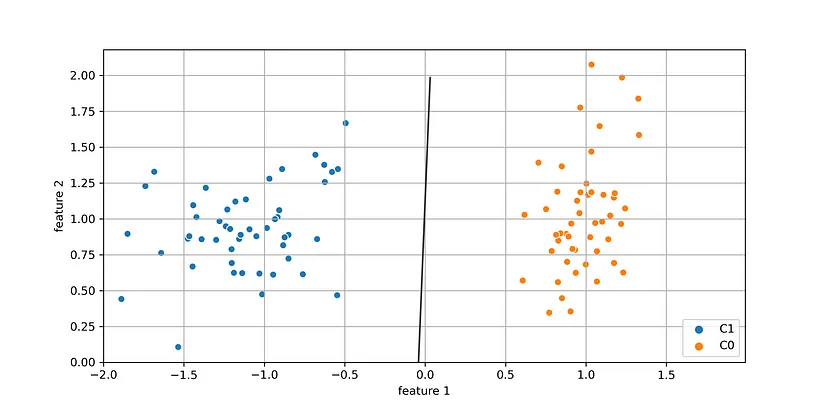
\includegraphics[width=0.6\textwidth]{pic/logisticR-Linear.png}
    %   % \label{fig:image}
    % \end{figure}
    \begin{itemize}
        \item Suppose we have a binary classification task (so $K=2$).
        \item By observing \textcolor{deepred}{age}, \textcolor{deepred}{gender}, \textcolor{deepred}{height}, \textcolor{deepred}{weight} and \textcolor{deepred}{BMI} we try to distinguish if a person is \textcolor{deepgreen}{overweight} or \textcolor{deepgreen}{not overweight}.
        
        
        %%%
        \begin{table}[h!]
        \centering
        \begin{tabular}{|c|c|c|c|c|c|}
        \hline
        \textcolor{deepred}{Age} & \textcolor{deepred}{Gender} & \textcolor{deepred}{Height (cm)} & \textcolor{deepred}{Weight (kg)} & \textcolor{deepred}{BMI} & \textcolor{deepgreen}{Overweight} \\ \hline
        25 & Male & 175 & 80 & 25.3 & 0 \\ \hline
        30 & Female & 160 & 60 & 22.5 & 0 \\ \hline
        \multicolumn{6}{|c|}{\dots} \\ \hline
        35 & Male & 180 & 90 & 27.3 & 1 \\ \hline
        \end{tabular}
        % \caption{Sample Table}
        % \label{tab:sample}
        \end{table}
        %%%%
        \item We denote the \textcolor{deepred}{features} of a sample with vector $x$ and the \textcolor{deepgreen}{label} with $y$.
        \item In logistic regression we try to find an $\sigma (\mathbf{w}^\top \mathbf{x})$ which predicts \textbf{posterior} probabilities $\mathbb{P}(y=1|\mathbf{x})$.
    \end{itemize}
    
\end{frame}
%%%% 5.1 %%%%%%%%%
\begin{frame}{Introduction (cont.)}
    \begin{itemize}
        \item $\sigma (\mathbf{w}^\top x)$: probability that $y=1$ given $x$ (parameterized by \textbf{$\textbf{w}$})
      \begin{align*}
        \mathbb{P}(y=1|\mathbf{x},\mathbf{w}) &= \sigma (\mathbf{w}^\top x) \\
        \mathbb{P}(y=0|\mathbf{x},\mathbf{w}) &= 1 - \sigma (\mathbf{w}^\top x)
      \end{align*}

        \item We need to look for a function which gives us an output in the range [0, 1]. (like a probability).

        \item Let's denote this function with $\sigma (.)$ and call it the \textbf{activation function}.
        
    \end{itemize}
\end{frame}

%%%% 6 %%%%%
\begin{frame}{Introduction (cont.)}
  \begin{minipage}{0.55\textwidth}
    \begin{itemize}
      \item Sigmoid (logistic) function:
      \[
        \sigma(z)=\frac{1}{1+e^{-z}}
      \]
      \item Smooth, bounded in $(0,1)$, and \textbf{differentiable}.
       \[
       \begin{aligned}
      \sigma'(z)=\frac{e^{-z}}{(1+e^{-z})^{2}}
      &=\underbrace{\frac{1}{1+e^{-z}}}_{\sigma(z)}\;
       \underbrace{\frac{e^{-z}}{1+e^{-z}}}_{1-\sigma(z)}
      \\ &=\sigma(z)\big(1-\sigma(z)\big)
      \end{aligned}
    \]
    \end{itemize}
   
  \end{minipage}\hfill
  \begin{minipage}{0.4\textwidth}
    \centering
    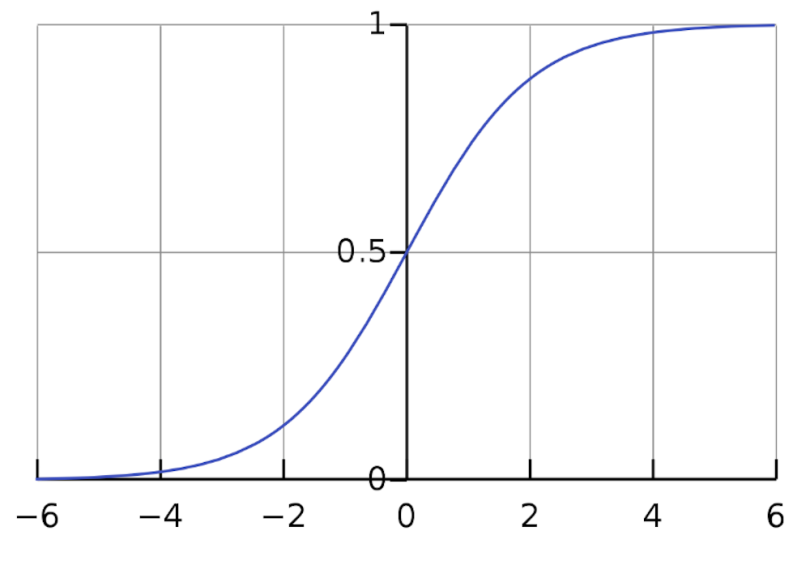
\includegraphics[width=0.8\linewidth]{pic/sigmoid.png}

    \vspace{0.5em}

    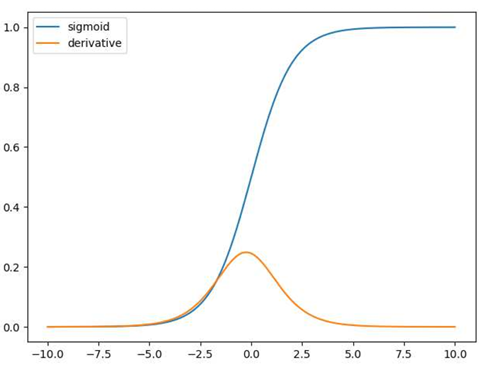
\includegraphics[width=0.8\linewidth]{pic/sigmoidDer.png}
  \end{minipage}
\end{frame}

%%%%%%%%%%%%%%%%%%%%%%%%%%%%%%%%%%%%%%%%
%%%% 7 %%%%
% \begin{frame}{Basics Cont.}
%     \begin{itemize}
%       \item Sigmoid function plot
%       \begin{figure}[h]
    
%       % \caption{Sigmoid plot}
%     % \label{fig:image}
%     \end{figure}
%     \end{itemize}
% \end{frame}
%%%% 8 %%%%%
\begin{frame}{Introduction (cont.)}
    \begin{itemize}
      \item The sigmoid function takes a number as input but we have:
    \end{itemize}
        \begin{align*}
            \mathbf{x} &= [x_0=1,x_1, \dots, x_d] \\
            \mathbf{w} &= [w_0, w_1, \dots, w_d]
        \end{align*}
    \begin{itemize} 
      \item So we can use the \textbf{dot product} of $\mathbf{x}$ and $\mathbf{w}$.
      
      \item We have $0\leq \sigma (\mathbf{w}^\top \mathbf{x}) \leq 1$. which is the estimated probability of $y=1$ on input $x$.

      \item An Example : A basketball game (Win, Lose)
        \begin{itemize}
            \item $\sigma (\mathbf{w}^\top  \mathbf{x}) = 0.7$
            \item In other terms $70$ percent chance of winning the game.
        \end{itemize}
        
    \end{itemize}
\end{frame}
%%%%% 9 %%%%%%%
\section{Decision surface}
\begin{frame}{Decision surface}
    \begin{itemize}
      \item Decision surface or decision boundary is the region of a problem space in which the output label of a classifier is ambiguous. (could be linear or non-linear)
      \item In binary classification it is where the probability of a sample belonging to each $y=0$ and $y=1$ is equal.
    \end{itemize}
    
    
     \begin{center}
        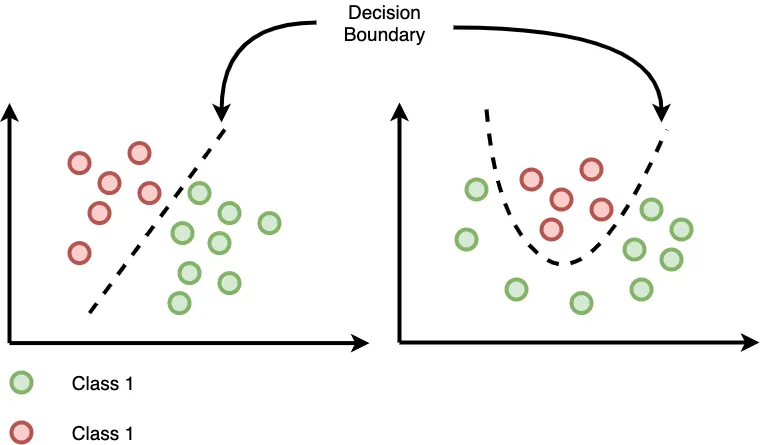
\includegraphics[width=0.4\textwidth]{pic/decision boundary.png}
        % \captionof{figure}{\footnotesize [Eric Xing, Machine Learning, CMU]}
    \end{center}
    
    \begin{itemize}
        
      \item Decision boundary hyperplane always has \textbf{one less dimension} than the feature space.
      
      
      %%% next slide
    %   \item an example of decision boundaries:
      
     
    \end{itemize}
\end{frame}
%%%%% 9.4 %%%%%%
\begin{frame}{Decision surface (cont.)}

    \begin{itemize}
        \item An example of linear decision boundaries:
    \end{itemize}
    \begin{center}
        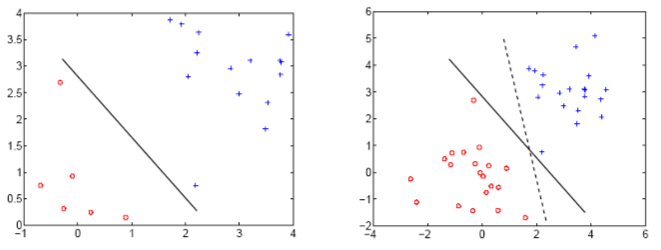
\includegraphics[width=0.85\textwidth]{pic/DBoundary.png}
        % \captionof{figure}{\footnotesize [Eric Xing, Machine Learning, CMU]}
    \end{center}
    \begin{tikzpicture}[remember picture,overlay]
        \node[anchor=south west, xshift=0.1cm, yshift=0.22cm] at (current page.south west) {
            \scriptsize Figure adapted from Eric Xing, Machine Learning, CMU
        };
    \end{tikzpicture}
\end{frame}
%%%% 9.5 %%%%%

\begin{frame}{Decision surface (cont.)}
    \begin{itemize}
      \item Back to our logistic regression problem.
      \item Decision surface $\sigma (\mathbf{w}^\top \mathbf{x}) = $ \textbf{constant}.
        \[
            \sigma (\mathbf{w}^\top \mathbf{x}) = \frac{1}{1 + e^{-(\mathbf{w}^\top \mathbf{x})}} = 0.5
        \]
      \item Decision surfaces are \textbf{linear functions} of $x$
        \begin{itemize}
            \item if $\sigma (\mathbf{w}^\top \mathbf{x}) \geq 0.5$ then $\hat{y}=1$, else $\hat{y} = 0$
            \item Equivalently, since $\sigma(z) \ge 0.5$ only when $z \ge 0$, this means:
            \begin{itemize}
                \item if $\mathbf{w}^\top \mathbf{x} \geq 0$ then decide $\hat{y}=1$, else $\hat{y}=0$
            \end{itemize}
        \end{itemize}% ayoub eshgh
        \vfill
        \begin{center}
            \( \hat{y} \) \textbf{is the predicted label}
        \end{center}
    \end{itemize}
\end{frame}

%%%% 10 %%%%
\begin{frame}{Decision boundary example}
    \begin{align*}
        \sigma (\mathbf{w}^\top \mathbf{x}) = \sigma (w_0 + w_1 x_1 + w_2 x_2)
    \end{align*}
    
    \begin{minipage}{0.35\linewidth}
        \centering
        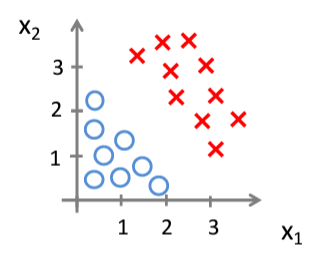
\includegraphics[width=\linewidth]{pic/lrDB1.png}
    \end{minipage}
    \hfill
    \begin{minipage}{0.35\linewidth}
        \centering
        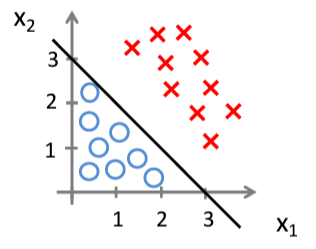
\includegraphics[width=\linewidth]{pic/lrDB2.png}
    \end{minipage}
    
    \begin{align*}
        \text{Predict } y=1 \text{ if } -3 + x_1 + x_2 \geq 0
    \end{align*}
    
\end{frame}
%%%%%%%%%%%%%
\begin{frame}{Non-linear decision boundary example}
    \begin{align*}
        \sigma (\mathbf{w}^\top \mathbf{x}) &= \sigma (w_0 + w_1 x_1 + w_2 x_2 + w_3x_1^2 + w_4x_2^2) \\
        \text{We can learn } & \text{more complex decision boundaries when having higher order terms}
    \end{align*}
    
    \begin{minipage}{0.30\linewidth}
        \centering
        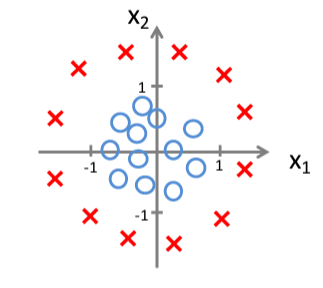
\includegraphics[width=\linewidth]{pic/lrDB3.png}
    \end{minipage}
    \hfill
    \begin{minipage}{0.30\linewidth}
        \centering
        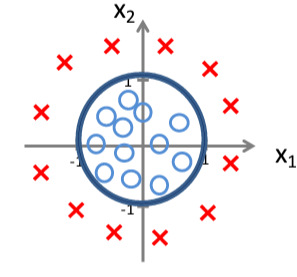
\includegraphics[width=\linewidth]{pic/lrDB4.png}
    \end{minipage}
    
    \begin{align*}
        \text{Predict } y=1 \text{ if } -1 + x_1^2 + x_2^2 \geq 0
    \end{align*}
    
\end{frame}
%%%%%%%%%%%%%

\section{MLE and MAP}

%%%%%%%%%%%%%%%%%%%%%%%%%%%%%%%%%%%%%%
\begin{frame}{Maximum Likelihood Estimation (MLE)}
    \begin{itemize}
        \item For $n$ independent samples, the likelihood is:
        \[
            \mathcal{L}(\mathbf{w}) = \prod_{i=1}^{n} \mathbb{P}(y^{(i)}|\mathbf{x}^{(i)}, \mathbf{w})
        \]
        \item For binary classification ($y \in \{0,1\}$):
        \[
            \mathbb{P}(y^{(i)}|\mathbf{x}^{(i)},\mathbf{w}) = \sigma (\mathbf{w}^\top \mathbf{x}^{(i)})^{y^{(i)}} (1 - \sigma (\mathbf{w}^\top \mathbf{x}^{(i)}))^{1 - y^{(i)}}
        \]
        \item This compact form works because $y^{(i)} \in \{0, 1\}$:
        \begin{itemize}
            \item If $y^{(i)}=1$, the expression becomes $P(y=1|\mathbf{x}^{(i)}, \mathbf{w}) = \sigma (\mathbf{w}^\top \mathbf{x}^{(i)})$.
            \item If $y^{(i)}=0$, the expression becomes $P(y=0|\mathbf{x}^{(i)}, \mathbf{w}) = 1 - \sigma (\mathbf{w}^\top \mathbf{x}^{(i)})$.
        \end{itemize}
        \item Log-likelihood:
        \[
            \log \mathcal{L}(\mathbf{w}) = \sum_{i=1}^n \big[ y^{(i)} \log \sigma(\mathbf{w}^\top \mathbf{x}^{(i)}) + (1-y^{(i)})\log (1-\sigma(\mathbf{w}^\top \mathbf{x}^{(i)})) \big]
        \]
    \end{itemize}
\end{frame}

%%%%%%%%%%%%%%%%%%%%%%%%%%%%%%%%%%%%%%
\begin{frame}{From Likelihood to Cost Function}
    \begin{itemize}
        \item Maximizing the likelihood $\Leftrightarrow$ minimizing the negative log-likelihood (NLL):
        \[
            J_{\text{MLE}}(\mathbf{w}) = -\log \mathcal{L}(\mathbf{w})
        \]
        \item Can be written as an integral over the data distribution:
        \[
            J_{\text{MLE}}(\mathbf{w}) = - \int \mathbb{P}(\mathbf{x},y) \log \mathbb{P}(y|\mathbf{x}, \mathbf{w}) \, d\mathbf{x}\,dy
        \]
        \item Empirical estimate (training data):
        \[
            J_{\text{MLE}}(\mathbf{w}) = -\frac{1}{n}\sum_{i=1}^{n} \log \mathbb{P}(y^{(i)}|\mathbf{x}^{(i)}, \mathbf{w})
        \]
        \item This is exactly the \textbf{cross-entropy loss} used in classification.
    \end{itemize}
\end{frame}

%%%%%%%%%%%%%%%%%%%%%%%%%%%%%%%%%%%%%%
\begin{frame}{Maximum A Posteriori Estimation (MAP)}
    \begin{itemize}
        \item MAP incorporates prior knowledge about parameters:
        \[
            \mathbf{w}_{\text{MAP}} = \arg\max_{\mathbf{w}}       \mathbb{P}(\mathbf{w}|D)
        \]
        \item Using Bayes’ rule:
        \[
            \mathbb{P}(\mathbf{w}|D) \propto P(D|\mathbf{w})P(\mathbf{w})
        \]
        \item Equivalently:
        \[
            \mathbf{w}_{\text{MAP}} = \arg\max_{\mathbf{w}} \Big[ \log \mathbb{P}(D|\mathbf{w}) + \log \mathbb{P}(\mathbf{w}) \Big]
        \]
        \item Cost function:
        \[
            J_{\text{MAP}}(\mathbf{w}) = - \sum_{i=1}^n \log \mathbb{P}(y^{(i)}|\mathbf{x}^{(i)}, \mathbf{w}) - \log \mathbb{P}(\mathbf{w})
        \]
    \end{itemize}
\end{frame}

%%%%%%%%%%%%%%%%%%%%%%%%%%%%%%%%%%%%%%
% \begin{frame}{MAP with Gaussian Prior (L2 Regularization)}
%     \begin{itemize}
%         \item Gaussian prior: $\mathbf{w} \sim \mathcal{N}(0, \tau^2 I)$
%         \[
%             P(\mathbf{w}) \propto \exp\left(-\frac{\|\mathbf{w}\|^2}{2\tau^2}\right)
%         \]
% \subsection{MLE and MAP}
%         \[
%             J_{\text{MAP}}(\mathbf{w}) = J_{\text{MLE}}(\mathbf{w}) + \frac{1}{2\tau^2}\|\mathbf{w}\|^2
%         \]
%         \item Let $\lambda = 1/\tau^2$:
%         \[
%             J_{\text{MAP}}(\mathbf{w}) = J_{\text{MLE}}(\mathbf{w}) + \frac{\lambda}{2}\|\mathbf{w}\|^2
%         \]
%         \item Equivalent to \textbf{L2-regularized logistic regression}.
%     \end{itemize}
% \end{frame}

%%%%%%%%%%%%%%%%%%%%%%%%%%%%%%%%%%%%%%
\begin{frame}{MAP with Gaussian Prior (L2 Regularization)}
    \begin{itemize}
        \item Gaussian prior: $\mathbf{w} \sim \mathcal{N}(0, \sigma^2 \mathbf{I})$
        \[
            \mathbb{P}(\mathbf{w}) \propto \exp\left(-\frac{\|\mathbf{w}\|_2^2}{2\sigma^2}\right)
        \]
        \item MAP cost:
        \[
            J_{\text{MAP}}(\mathbf{w}) = J_{\text{MLE}}(\mathbf{w}) + \lambda \|\mathbf{w}\|_2^2
        \]
        \item L2 penalty encourages \textbf{weight shrinkage} (smooth regularization, no sparsity).
    \end{itemize}
\end{frame}


%%%%%%%%%%%%%%%%%%%%%%%%%%%%%%%%%%%%%%
\begin{frame}{MAP with Laplace Prior (L1 Regularization)}
    \begin{itemize}
        \item Laplace prior: $\mathbf{w} \sim \text{Laplace}(0, b)$
        \[
            \mathbb{P}(\mathbf{w}) \propto \exp\left(-\frac{\|\mathbf{w}\|_1}{b}\right)
        \]
        \item MAP cost:
        \[
            J_{\text{MAP}}(\mathbf{w}) = J_{\text{MLE}}(\mathbf{w}) + \lambda \|\mathbf{w}\|_1
        \]
        \item L1 penalty encourages \textbf{sparsity} (feature selection).
    \end{itemize}
\end{frame}

%%%%%%%%%%%%%%%%%%%%%%%%%%%%%%%%%%%%%%
\begin{frame}{Ridge vs. Lasso (Recap)}
        \begin{table}[h!]
        \centering
        \renewcommand{\arraystretch}{1.4}
        \setlength{\tabcolsep}{8pt}
        \begin{tabular}{|p{0.45\textwidth}|p{0.45\textwidth}|}
            \hline
            \textbf{Ridge Regression (L2)} & \textbf{Lasso Regression (L1)} \\
            \hline
            Constraint: $\|\mathbf{w}\|_2^2 \le t$ (L2 ball). &
            Constraint: $\|\mathbf{w} \|_1 \le t$ (L1 ball). \\
            \hline
            Contours of $J(\mathbf{w})$ typically touch the constraint boundary at smooth points. &
            Contours often hit the sharp \textbf{corners} of the diamond. \\
            \hline
            Produces small but nonzero coefficients (no exact sparsity). &
            Produces \textbf{sparse} solutions (some coefficients exactly zero). \\
            \hline
            Differentiable everywhere; the regularizer $\|\mathbf{w}\|_2^2$ is smooth. &
            Not differentiable at $w_i = 0$; $\|\mathbf{w}\|_1$ has sharp corners. \\
            \hline
            Strongly convex $\Rightarrow$ guarantees a \textbf{unique optimum}. &
            Not strongly convex $\Rightarrow$ may yield \textbf{multiple optima}. \\
            \hline
        \end{tabular}
    \end{table}
\end{frame}

%%%% 12 %%%%%%

\section{Gradient descent}
\begin{frame}{Gradient descent}
    \begin{itemize}
    \item Remember from previous slides:
        \[
        J(\mathbf{w}) = \sum_{i=1}^{n}-y^{(i)}\log (\sigma (\mathbf{w}^\top  \mathbf{x}^{(i)})) - 
            (1-y^{(i)})\log (1 - \sigma (\mathbf{w}^\top  \mathbf{x}^{(i)}))
        \]
    \item Update rule for \textbf{gradient descent}: 
        \begin{align*}
            \mathbf{w}^{t+1} = \mathbf{w}^t - \eta \nabla_{\mathbf{w}} J(\mathbf{w}^t)
        \end{align*}
    \item With $J(\mathbf{w})$ definition for logistic regression we get:
    \[
    \nabla_\mathbf{w} J(\mathbf{w})
    = \sum_{i=1}^{n} (\sigma(\mathbf{w}^\top \mathbf{x}^{(i)}) - y^{(i)})\mathbf{x}^{(i)}
    \]
    % \item Also keep in mind $f(x^{(i)}; \mathbf{w})= \sigma (\mathbf{w}^\top x^{(i)})$
    % \item Compare with the gradient of \textbf{SSE} in \textbf{linear regression} :
    %     \begin{align*}
    %         \nabla _w J(w) = \sum_{i=1}^{n} (\mathbf{w}^\top x^{(i)} - y^{(i)})x^{(i)}
    %     \end{align*}
        
    \end{itemize}
\end{frame}

\begin{frame}{Gradient descent (cont.)}
Let's find the derivative from the previous slide step by step:
    \begin{itemize}
        \item For one sample, we have:
        \[
        J_i = -y^{(i)}\log\sigma(z^{(i)}) - (1 - y^{(i)})\log(1 - \sigma(z^{(i)})), 
        \quad z^{(i)} = \mathbf{w}^\top \mathbf{x}^{(i)}
        \]
        \item Differentiate w.r.t. \(z^{(i)}\):
        \[
        \frac{\partial J_i}{\partial z^{(i)}} 
        = -\frac{y^{(i)}}{\sigma(z^{(i)})}\sigma'(z^{(i)}) 
        + \frac{1 - y^{(i)}}{1 - \sigma(z^{(i)})}\sigma'(z^{(i)})
        = \sigma(z^{(i)}) - y^{(i)}
        \]
        \item By chain rule we get:
        \[
        \frac{\partial J_i}{\partial \mathbf{w}} = 
        \frac{\partial J_i}{\partial z^{(i)}} \cdot \frac{\partial z^{(i)}}{\partial \mathbf{w}} = (\sigma(z^{(i)}) - y^{(i)})\,\mathbf{x}^{(i)}
        \]
        \item Summing over all samples gives the result:
        \[
        \nabla_{\mathbf{w}} J(\mathbf{w}) 
        = \sum_{i=1}^{n} (\sigma(\mathbf{w}^\top \mathbf{x}^{(i)}) - y^{(i)})\,\mathbf{x}^{(i)}
        \]
    \end{itemize}
\end{frame}


%%%%%% 12.5 %%%%%%%
\begin{frame}{Gradient descent (cont.)}
    \begin{itemize}
    
    \item Compare the gradient of \textcolor{deepgreen}{logistic regression} with the gradient of \textcolor{blue}{SSE} in \textcolor{blue}{linear regression} :
    \end{itemize}
        \begin{align*}
        \color{deepgreen}
             \nabla_{\mathbf{w}} J(\mathbf{w}) = \sum_{i=1}^{n} (\sigma (\mathbf{w}^\top \mathbf{x}^{(i)}) - y^{(i)})\mathbf{x}^{(i)} 
        \end{align*}
        \begin{align*}
            \color{blue}
            \nabla_{\mathbf{w}} J(\mathbf{w}) = \sum_{i=1}^{n} (\mathbf{w}^\top \mathbf{x}^{(i)} - y^{(i)})\mathbf{x}^{(i)}
        \end{align*}
        
\end{frame}
%%%%% 13 %%%%%%%%
\begin{frame}{Loss function}
    \begin{itemize}
        \item Loss function is a single overall measure of loss incurred for taking our decisions (over entire dataset).
        \item This is the \textbf{cross-entropy} (or log) loss for a single sample:
        \[ J(y, \sigma (\mathbf{w}^\top  \mathbf{x})) = -y \log (\sigma ( \mathbf{w}^\top  \mathbf{x})) - (1-y) \log 
        (1 - \sigma (\mathbf{w}^\top  \mathbf{x}))
        \]
        
        \item Since in binary classification $y \in \{0, 1\}$, the loss simplifies:
            \[
                J(y, \sigma (\mathbf{w}^\top  \mathbf{x})) = \begin{cases}
                    - \log (\sigma (\mathbf{w}^\top  \mathbf{x})) & \textbf{if } y = 1 \\
                    - \log (1 - \sigma (\mathbf{w}^\top  \mathbf{x})) & \textbf{if } y = 0
                \end{cases}
            \]
    \end{itemize}
\end{frame}

%%%%% 14 %%%%%%%%
\begin{frame}{Convexity of Cross-Entropy Loss}
\small
This is the logistic regression loss over the dataset:
\[
J(\mathbf{w}) = \sum_{i=1}^{n} \Big[ -y^{(i)} \log \sigma(\mathbf{w}^\top \mathbf{x}^{(i)}) - (1 - y^{(i)}) \log(1 - \sigma(\mathbf{w}^\top \mathbf{x}^{(i)})) \Big],
\]
Define $\hat{y}^{(i)} = \sigma(\mathbf{w}^\top \mathbf{x}^{(i)})$.  
Then the gradient is:
\[
\nabla_{\mathbf{w}} J(\mathbf{w}) = \sum_{i=1}^{n} (\hat{y}^{(i)} - y^{(i)}) \, \mathbf{x}^{(i)}.
\]
The Hessian (second derivative matrix) is:
\[
\nabla_{\mathbf{w}}^2 J(\mathbf{w}) = \sum_{i=1}^{n} \hat{y}^{(i)}(1 - \hat{y}^{(i)}) \, \mathbf{x}^{(i)} (\mathbf{x}^{(i)})^\top
= \mathbf{X}^\top \mathbf{D} \, \mathbf{X},
\]
where $\mathbf{D} = \mathrm{diag}(\hat{y}^{(i)}(1 - \hat{y}^{(i)}))$ and each $\hat{y}^{(i)}(1 - \hat{y}^{(i)}) \ge 0$.
For any vector $\mathbf{v}$,
\[
\mathbf{v}^\top \nabla_{\mathbf{w}}^2 J(\mathbf{w}) \, \mathbf{v} 
= \sum_{i=1}^{n} \hat{y}^{(i)}(1 - \hat{y}^{(i)}) \, (\mathbf{v}^\top \mathbf{x}^{(i)})^2 \ge 0.
\]
Hence, the Hessian is \textbf{positive semidefinite (PSD)}, and $J(\mathbf{w})$ is \textbf{convex}.
\end{frame}



%%%%% 13.5 %%%%%%%%
\begin{frame}{Loss function (cont.)}
    \begin{itemize}
        \item Note that this is different from the \textbf{zero-one loss}, which simply counts misclassifications:
           \[
               J_{0-1}(y, \hat{y}) =  \begin{cases}
                    1 & \textbf{if } y \neq \hat{y} \\
                    0 & \textbf{if } y = \hat{y}
                \end{cases}
            \]
            ($\hat{y}$ is the predicted label and $y$ is the true label)
            
        \item We use cross-entropy (logistic loss) instead of zero-one loss because the zero-one loss function is \textbf{non-differentiable} and \textbf{non-convex}. 
        
        \item The cross-entropy loss is a smooth, convex, and differentiable substitute, which allows us to use optimization methods like gradient descent.
    \end{itemize}
\end{frame}
%%%%% 14 %%%%%%
% \begin{frame}{Cost Function Summary}
%     \begin{itemize}
%         \item Logistic regression (LR) has a more proper cost function for classification than SSE and Perceptron.

%         \item Why is the cost function of LR also more suitable than 
%             \begin{align*}
%                 J(w) = \frac{1}{n}\sum_{i=1}^{n}(y^{(i)} - f(x^{(i)}; \mathbf{w}))^2
%             \end{align*}
%         Where $f(x; \mathbf{w}) = \sigma(\mathbf{w}^\top x)$?
%             \begin{itemize}
%                 \item The conditional distribution $p(y|x, \mathbf{w})$ in the classification problem is not Guassian (it is \textbf{Bernoulli}).
%                 \item The cost function of LR is also convex.
%             \end{itemize}
%     \end{itemize}
% \end{frame}

%%%%%% 15 %%%%%%%

\section{Multi-class logistic regression}
\begin{frame}{Multi-class logistic regression}
    \begin{itemize}
        \item Now consider a problem where we have $K$ classes and every sample only belongs to one class (for simplicity).
        % \item For each class $k$, $f_k(x; \mathbf{W})$ predicts the probability of $y=k$.
        %     \begin{itemize}
        %         \item i.e., $P(y=k|x, \mathbf{W})$
        %     \end{itemize}
        % \item For each data point $x_0$, $\sum _{k=1}^{K} p(y=k|x_0, \mathbf{W})$ must be $1$
        %     \begin{itemize}
        %         \item $W$ denotes a matrix of $w_i$'s in which each $w_i$ is a weight vector dedicated for class label $i$.
        %     \end{itemize}
        % \item On a new input $x$, to make a prediction, we pick the class that maximizes $f_k(x; \mathbf{W})$:
        %     \begin{align*}
        %         \alpha (x) &= \underset{k=1, \dots , K}{\arg\max} \hspace{0.2cm} f_k(x) 
        %     \end{align*}
        %     \begin{center}
        %         \textbf{if $\color{red} f_k(x) > f_j(x)$ $\color{red} \forall j \neq k$ then decide $\color{red} C_k$}
        %     \end{center}
    \end{itemize}
    \centering
    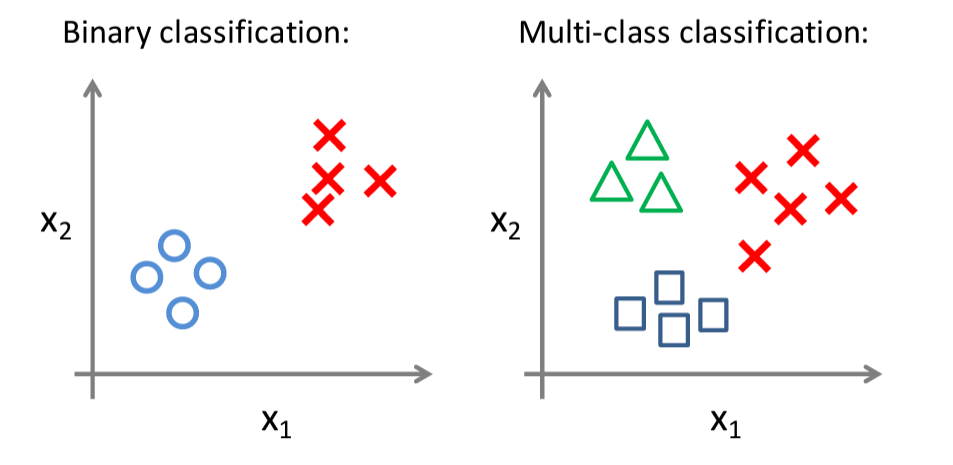
\includegraphics[width=0.8 \linewidth]{pic/multiVsBinaryC.png}
\end{frame}
%%%%%%%%%%%%%%%%%%%%%%%%
\begin{frame}{Multi-class logistic regression (cont.)}
    \begin{itemize}
         \item For each class $k$, $\sigma _k(\mathbf{x}; \mathbf{W})$ predicts the probability of $y=k$.
            \begin{itemize}
                \item i.e., $\mathbb{P}(y=k|\mathbf{x}, \mathbf{W})$
            \end{itemize}
        \item For each data point $\mathbf{x}$, $\sum _{k=1}^{K} \mathbb{P}(y=k|\mathbf{x}, \mathbf{W})$ must be $1$
            \begin{itemize}
                \item $\mathbf{W}$ denotes a matrix of $\mathbf{w}_i$'s in which each $\mathbf{w}_i$ is a weight vector dedicated for class label $i$.
            \end{itemize}
        \item On a new input $x$, to make a prediction, we pick the class that maximizes $\sigma _k(\mathbf{x}; \mathbf{W})$:
            \begin{align*}
                \alpha (\mathbf{x}) &= \underset{k=1, \dots , K}{\arg\max} \hspace{0.2cm} \sigma _k(\mathbf{x}; \mathbf{W}) 
            \end{align*}
            \begin{center}
                \textbf{if $\color{red} \sigma _k(\mathbf{x}; \mathbf{W}) > \sigma _j(\mathbf{x}; \mathbf{W})$ $\color{red} \forall j \neq k$ then decide $\color{red} C_k$}
            \end{center}
    \end{itemize}
\end{frame}


%%%%% 16 %%%%%%%
\begin{frame}{Multi-class logistic regression (cont.)}
    \begin{itemize}
        \item $K > 2$ and $y \in \{1,2,\dots,K\}$
        \begin{align*}
            \sigma _k(\mathbf{x}, \mathbf{W}) = \mathbb{P}(y=k|\mathbf{x}) = \frac{\exp{(\mathbf{w}^\top _k\mathbf{x})}}{\sum_{j=1}^{K}\exp{(\mathbf{w}_j^\top\mathbf{x})}}
        \end{align*}
        \item Normalized exponential (Aka \textbf{Softmax})
          
            \item if $\mathbf{w}_k^\top \mathbf{x} \gg \mathbf{w}_j^\top \mathbf{x}$ for all $j \neq k$ then $\mathbb{P}(C_k|\mathbf{x}) \approx 1$ and $\mathbb{P}(C_j|x) \approx 0$
            \item Note : remember from Bayes theorem:
                \[
                \mathbb{P}(C_k|x) = \frac{\mathbb{P}(\mathbf{x}|C_k)\mathbb{P}(C_k)}
            {\sum_{j=1}^{K}\mathbb{P}(\mathbf{x}|C_j)\mathbb{P}(C_j)}
                \]
          
    \end{itemize}
\end{frame}
%%%%% 16.5 %%%%%
\begin{frame}{Multi-class logistic regression (cont.)}
    \begin{itemize}
        \item Softmax function \textbf{smoothly} highlights the maximum probability and is differentiable.
        \item Compare it with $\max (.)$ function which is strict and non-differentiable
        \item Softmax can also handle negative values because we are using exponential function
        \item And it gives us probability for each class since:
            \begin{align*}
                \displaystyle \sum _{k=1}^{K} \frac{\exp (\mathbf{w}_k^\top \mathbf{x})}{\sum _{j=1}^{K} \exp (\mathbf{w}_j^\top \mathbf{x}) } = 1
            \end{align*}
    \end{itemize}
\end{frame}

%%%% 16.6 %%%%%
\begin{frame}{Multi-class logistic regression (cont.)}
    \begin{itemize}
        \item An example of applying softmax (note that $z_i=\mathbf{w}^\top \mathbf{x}^{(i)}$):
    \end{itemize}
    \begin{center}
        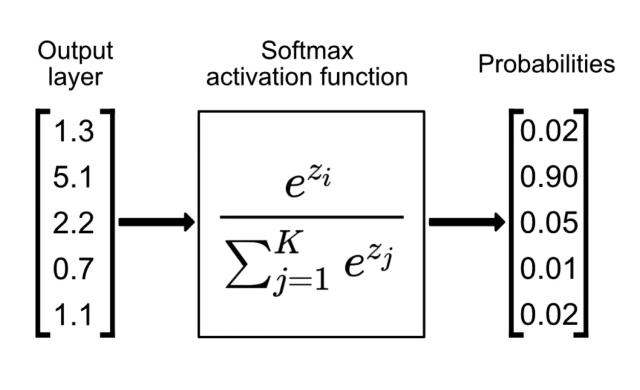
\includegraphics[width=0.7\textwidth]{pic/softmax0.png}
       
    \end{center}
\end{frame}

%%%% 17 %%%%%
\begin{frame}{Multi-class logistic regression (cont.)}
    \begin{itemize}
        \item Again we set $J(\mathbf{W})$ as negative of log likelihood.
        \item We need $\mathbf{W}_{\text{MLE}} = \underset{\mathbf{W}}{\arg\min} \hspace{0.2cm} J(\mathbf{W})$
        \begin{align*}
            J(W) &= -\log \prod_{i=1}^{n} \textcolor{red}{\mathbb{P}(\mathbf{y}^{(i)}|\mathbf{x}^{(i)}, \mathbf{W})} \\
            &= -\log \prod_{i=1}^{n}\textcolor{red}{\prod_{k=1}^{K}\sigma _k(\mathbf{x}^{(i)}; \mathbf{W})^{y_k^{(i)}} }\\
            &= -\sum_{i=1}^{n}\sum_{k=1}^{K}y_k^{(i)} \log (\sigma _k(\mathbf{x}^{(i)}; \mathbf{W}))
        \end{align*}
        \item If \textbf{$\textbf{i}$-th} sample belongs to class $k$ then $y^{(i)}_k$ is 1 else 0.
        \item Again no closed-from solution for $\mathbf{W_{\text{MLE}}}$
    \end{itemize}
    
\end{frame}
%%%%%%% 17.5 %%%%%%%
\begin{frame}{Multi-class logistic regression (cont.)}
    \begin{itemize}
        \item From previous slides we have:
            \begin{align*}
                J(\mathbf{W}) = -\sum_{i=1}^{n}\sum_{k=1}^{K}y_k^{(i)} \log (\sigma _k(\mathbf{x}^{(i)}; \mathbf{W}))
            \end{align*}
        \item In which:
             \[
        \mathbf{W} = [\mathbf{w}_1,\mathbf{w}_2, \dots, \mathbf{w}_K], \quad \mathbf{Y} = 
        \text{\small $
        \begin{pmatrix}
            \mathbf{y}^{(1)} \\
            \mathbf{y}^{(2)} \\
            \vdots \\
            \mathbf{y}^{(n)}
        \end{pmatrix}
        $}
        =
        \begin{pmatrix}
            y_1^{(1)} & \dots & y_K^{(1)} \\
            y_1^{(2)} & \dots & y_K^{(2)} \\
            \vdots    & \ddots & \vdots \\
            y_1^{(n)} & \dots & y_K^{(n)}
        \end{pmatrix}
    \]
    
        \item $\mathbf{y}$ is a vector of length $K$ (1-of-$K$ encoding)
            \begin{itemize}
                % \item Each vector $y^{(i)}$ only consists of zeros and ones.
                \item For example $\mathbf{y}=[0,0,1,0]^\top$ when the target class is $C_3$.
            \end{itemize}
    \end{itemize}
\end{frame}
%%%%%% 18 %%%%%%%%
\begin{frame}{Multi-class logistic regression (cont.)}
    \begin{itemize}
        \item Update rule for gradient descent:
        
    \end{itemize}
    \begin{align*}
            \mathbf{w}_j^{t+1} &= \mathbf{w}_j^t - \eta \nabla _{\mathbf{W}} J(\mathbf{W}^t) \\
            \nabla _{\mathbf{w}_{j}} J(\mathbf{W}) &= \sum_{i=1}^{n} (\sigma _j(\mathbf{x}^{(i)}; \mathbf{W}) - y_j^{(i)})\mathbf{x}^{(i)}
        \end{align*}
        
    \begin{itemize}
        \item $\mathbf{w}_j^t$ denotes the weight vector for class $j$ (since in multi-class LR, each class has its own weight vector) in the $t$-th iteration
    \end{itemize}
\end{frame}


% \section{Evaluation Metrics}

% \begin{frame}{Evaluation Context}
%     \begin{itemize}
%         \item Model evaluation quantifies predictive performance on unseen data.
%         \item Metrics are derived from the confusion matrix:
%     \end{itemize}
%     \vspace{0.3cm}
%     \begin{center}
%     \begin{tabular}{c|cc}
%         \toprule
%         & Predicted Positive & Predicted Negative \\
%         \midrule
%         Actual Positive & TP & FN \\
%         Actual Negative & FP & TN \\
%         \bottomrule
%     \end{tabular}
%     \end{center}
%     \vspace{0.3cm}
%     \begin{itemize}
%         \item TP, TN, FP, FN provide the foundation for classification performance indices.
%     \end{itemize}
% \end{frame}

% \begin{frame}{Accuracy and Error Rate}
%     \textbf{Accuracy:} proportion of correctly classified instances
%     \[
%         \text{Accuracy} = \frac{TP + TN}{TP + TN + FP + FN}
%     \]

%     \textbf{Error Rate:} complement of accuracy
%     \[
%         \text{Error Rate} = \frac{FP + FN}{TP + TN + FP + FN} = 1 - \text{Accuracy}
%     \]

%     \vspace{0.3cm}
%     \begin{itemize}
%         \item Accuracy is reliable for balanced class distributions.
%         \item Limited interpretability for skewed datasets.
%     \end{itemize}
% \end{frame}

% \begin{frame}{Precision and Recall}
%     \textbf{Precision (Positive Predictive Value)}
%     \[
%         P = \frac{TP}{TP + FP}
%     \]
%     \begin{itemize}
%         \item Fraction of predicted positives that are truly positive.
%         \item Sensitive to false positives.
%     \end{itemize}

%     \vspace{0.3cm}
%     \textbf{Recall (Sensitivity / True Positive Rate)}
%     \[
%         R = \frac{TP}{TP + FN}
%     \]
%     \begin{itemize}
%         \item Fraction of actual positives correctly identified.
%         \item Sensitive to false negatives.
%     \end{itemize}
% \end{frame}

% \begin{frame}{F1-Score and Trade-Off Analysis}
%     \textbf{F1-Score:} harmonic mean of precision and recall
%     \[
%         F1 = 2 \cdot \frac{P \cdot R}{P + R}
%     \]

%     \vspace{0.3cm}
%     \begin{itemize}
%         \item Provides a single measure balancing precision and recall.
%         \item Useful in imbalanced datasets or when both types of error are significant.
%         \item Trade-off: Increasing recall typically decreases precision and vice versa.
%     \end{itemize}
% \end{frame}

% \begin{frame}{Comparative Overview}
%     \begin{center}
%     \begin{tabular}{lccc}
%         \toprule
%         Metric & Formula & Focus & Typical Use-Case \\
%         \midrule
%         Accuracy & $\frac{TP+TN}{TP+FP+FN+TN}$ & Overall correctness & Balanced classes \\
%         Precision & $\frac{TP}{TP+FP}$ & False positive control & Spam detection, IR \\
%         Recall & $\frac{TP}{TP+FN}$ & False negative control & Medical diagnosis, anomaly detection \\
%         F1-Score & $2\frac{PR}{P+R}$ & Balance & Imbalanced or skewed datasets \\
%         \bottomrule
%     \end{tabular}
%     \end{center}
%     \vspace{0.3cm}
%     \begin{itemize}
%         \item Metric choice should reflect operational objectives and misclassification costs.
%         \item Always interpret metrics in conjunction with the confusion matrix.
%     \end{itemize}
% \end{frame}


% \section{Methods}

% \subsection{Diffusion Model}

% \begin{frame}{Title}
%     \begin{itemize}
%         \item \lipsum[3][1-4]
%     \end{itemize}
%     \begin{table}[h]
%         \centering
%         \begin{tabular}{c|c}
%             Microsoft\textsuperscript{\textregistered}  Windows & Apple\textsuperscript{\textregistered}  Mac OS \\
%             \hline
%             Windows-Kernel & Unix-like \\
%             Arm, Intel & Intel, Apple Silicon \\
%             Sudden update & Stable update \\
%             Less security & More security \\
%             ... & ... \\
%         \end{tabular}
%     \end{table}
% \end{frame}

% \begin{frame}{Algorithms}
%     \begin{exampleblock}{Non-Numbering Formula}
%         \begin{equation*}
%             J(\theta) = \mathbb{E}_{\pi_\theta}[G_t] = \sum_{s\in\mathcal{S}} d^\pi (s)V^\pi(s)=\sum_{s\in\mathcal{S}} d^\pi(s)\sum_{a\in\mathcal{A}}\pi_\theta(a|s)Q^\pi(s,a)
%         \end{equation*}
%     \end{exampleblock}
%     \begin{exampleblock}{Multi-Row Formula\footnote{If text appears in the formula,use $\backslash$mathrm\{\} or $\backslash$text\{\} instead}}
%         \begin{align}
%             Q_\mathrm{target}&=r+\gamma Q^\pi(s^\prime, \pi_\theta(s^\prime)+\epsilon)\\
%             \epsilon&\sim\mathrm{clip}(\mathcal{N}(0, \sigma), -c, c)\nonumber
%         \end{align}
%     \end{exampleblock}
% \end{frame}

% \begin{frame}
%     \begin{exampleblock}{Numbered Multi-line Formula}
%         % Taken from Mathmode.tex
%         \begin{multline}
%             A=\lim_{n\rightarrow\infty}\Delta x\left(a^{2}+\left(a^{2}+2a\Delta x+\left(\Delta x\right)^{2}\right)\right.\label{eq:reset}\\
%             +\left(a^{2}+2\cdot2a\Delta x+2^{2}\left(\Delta x\right)^{2}\right)\\
%             +\left(a^{2}+2\cdot3a\Delta x+3^{2}\left(\Delta x\right)^{2}\right)\\
%             +\ldots\\
%             \left.+\left(a^{2}+2\cdot(n-1)a\Delta x+(n-1)^{2}\left(\Delta x\right)^{2}\right)\right)\\
%             =\frac{1}{3}\left(b^{3}-a^{3}\right)
%         \end{multline}
%     \end{exampleblock}
% \end{frame}

% \begin{frame}{Graphics and Columns}
%     \begin{minipage}[c]{0.3\linewidth}
%         \psset{unit=0.8cm}
%         \begin{pspicture}(-1.75,-3)(3.25,4)
%             \psline[linewidth=0.25pt](0,0)(0,4)
%             \rput[tl]{0}(0.2,2){$\vec e_z$}
%             \rput[tr]{0}(-0.9,1.4){$\vec e$}
%             \rput[tl]{0}(2.8,-1.1){$\vec C_{ptm{ext}}$}
%             \rput[br]{0}(-0.3,2.1){$\theta$}
%             \rput{25}(0,0){%
%             \psframe[fillstyle=solid,fillcolor=lightgray,linewidth=.8pt](-0.1,-3.2)(0.1,0)}
%             \rput{25}(0,0){%
%             \psellipse[fillstyle=solid,fillcolor=yellow,linewidth=3pt](0,0)(1.5,0.5)}
%             \rput{25}(0,0){%
%             \psframe[fillstyle=solid,fillcolor=lightgray,linewidth=.8pt](-0.1,0)(0.1,3.2)}
%             \rput{25}(0,0){\psline[linecolor=red,linewidth=1.5pt]{->}(0,0)(0.,2)}
% %           \psRotation{0}(0,3.5){$\dot\phi$}
% %           \psRotation{25}(-1.2,2.6){$\dot\psi$}
%             \psline[linecolor=red,linewidth=1.25pt]{->}(0,0)(0,2)
%             \psline[linecolor=red,linewidth=1.25pt]{->}(0,0)(3,-1)
%             \psline[linecolor=red,linewidth=1.25pt]{->}(0,0)(2.85,-0.95)
%             \psarc{->}{2.1}{90}{112.5}
%             \rput[bl](.1,.01){C}
%         \end{pspicture}
%     \end{minipage}\hspace{2cm}
%     \begin{minipage}{0.5\linewidth}
%         \medskip
%         % \hspace{2cm}
%         \begin{figure}[h]
%             \centering
%             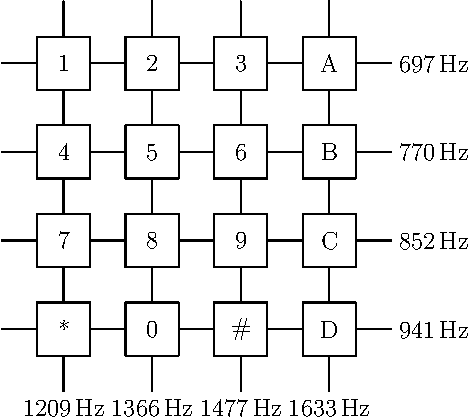
\includegraphics[height=.4\textheight]{pic/sample.pdf}
%         \end{figure}
%     \end{minipage}
% \end{frame}

% \begin{frame}[fragile]{\LaTeX{} Common Commands}
%     \begin{exampleblock}{Commands}
%         \centering
%         \footnotesize
%         \begin{tabular}{llll}
%             \cmd{chapter} & \cmd{section} & \cmd{subsection} & \cmd{paragraph} \\
%             chapter & section & sub-section & paragraph \\\hline
%             \cmd{centering} & \cmd{emph} & \cmd{verb} & \cmd{url} \\
%             center & emphasize & original & hyperlink \\\hline
%             \cmd{footnote} & \cmd{item} & \cmd{caption} & \cmd{includegraphics} \\
%             footnote & list item & caption & insert image \\\hline
%             \cmd{label} & \cmd{cite} & \cmd{ref} \\
%             label & citation & refer\\\hline
%         \end{tabular}
%     \end{exampleblock}
%     \begin{exampleblock}{Environment}
%         \centering
%         \footnotesize
%         \begin{tabular}{lll}
%             \env{table} & \env{figure} & \env{equation}\\
%             table & figure & formula \\\hline
%             \env{itemize} & \env{enumerate} & \env{description}\\
%             non-numbering item & numbering item & description \\\hline
%         \end{tabular}
%     \end{exampleblock}
% \end{frame}

% \begin{frame}[fragile]{\LaTeX{} Examples of environmental commands}
%     \begin{minipage}{0.5\linewidth}
% \begin{lstlisting}[language=TeX]
% \begin{itemize}
%   \item A \item B
%   \item C
%   \begin{itemize}
%     \item C-1
%   \end{itemize}
% \end{itemize}
% \end{lstlisting}
%     \end{minipage}\hspace{1cm}
%     \begin{minipage}{0.3\linewidth}
%         \begin{itemize}
%             \item A
%             \item B
%             \item C
%             \begin{itemize}
%                 \item C-1
%             \end{itemize}
%         \end{itemize}
%     \end{minipage}
%     \medskip
%     \pause
%     \begin{minipage}{0.5\linewidth}
% \begin{lstlisting}[language=TeX]
% \begin{enumerate}
%   \item A \item B
%   \item C
%   \begin{itemize}
%     \item[n+e]
%   \end{itemize}
% \end{enumerate}
% \end{lstlisting}
%     \end{minipage}\hspace{1cm}
%     \begin{minipage}{0.3\linewidth}
%         \begin{enumerate}
%             \item A
%             \item B
%             \item C
%             \begin{itemize}
%                 \item[n+e]
%             \end{itemize}
%         \end{enumerate}
%     \end{minipage}
% \end{frame}

% \begin{frame}[fragile]{\LaTeX{} Formulas}
%     \begin{columns}
%         \begin{column}{.55\textwidth}
% \begin{lstlisting}[language=TeX]
% $V = \frac{4}{3}\pi r^3$

% \[
%   V = \frac{4}{3}\pi r^3
% \]

% \begin{equation}
%   \label{eq:vsphere}
%   V = \frac{4}{3}\pi r^3
% \end{equation}
% \end{lstlisting}
%         \end{column}
%         \begin{column}{.4\textwidth}
%             $V = \frac{4}{3}\pi r^3$
%             \[
%                 V = \frac{4}{3}\pi r^3
%             \]
%             \begin{equation}
%                 \label{eq:vsphere}
%                 V = \frac{4}{3}\pi r^3
%             \end{equation}
%         \end{column}
%     \end{columns}
%     \begin{itemize}
%         \item more information \href{https://ja.overleaf.com/learn/latex/Mathematical_expressions}{\color{purple}{here}}
%     \end{itemize}
%%%%%%%%%%%%%%%%%%%%%%%%%%%%%%%%%%%%%%%%%%%%%%%%
\section{References}

\begin{frame}{Contributions}
\begin{itemize}
\item \textbf{These slides are authored by:}
\begin{itemize}
    \setlength{\itemsep}{5pt} % Adjust the value to control the spacing
    \item \href{https://github.com/alirezamirrokni}{Alireza Mirrokni}
    \item \href{https://github.com/Danial-Gharib}{Danial Gharib}
    \item {Amir Malek Hosseini}
    \item {Aida Jalali}
\end{itemize}
\end{itemize}

\end{frame}

\begin{frame}[allowframebreaks]
    \bibliography{ref}
    \bibliographystyle{ieeetr}
    \nocite{*}
\end{frame}

\end{document}
